%% -*- Lecture -*-

\documentclass[11pt,aspectratio=169]{beamer}

\usepackage{rcstalk}
\usepackage{bytefield}

\usetheme{rcstheme}

\subtitle{Lecture 8: Virtual Memory OS}
\topic{Virtual memory OS}

\usetikzlibrary{arrows, calc, shapes.geometric, shapes.misc,
    fit, chains, intersections, backgrounds, positioning}

\tikzset{
    colornode/.style={ fill=few-#1!67 },
}

\begin{document}

\maketitle

\newcommand{\descbox}[2]{\parbox[c][3.8\baselineskip]{0.95\width}{%
	\raggedright #1\vfill #2}}
\newcommand{\memsection}[4]{%
	% define the height of the memsection
	\bytefieldsetup{bitheight=#3\baselineskip}%
	\bitbox[]{10}{%
		\texttt{#1}%print end address
		\\
		% do some spacing
		\vspace{#3\baselineskip}
		\vspace{-2\baselineskip}
		\vspace{-#3pt}
		\texttt{#2}%print start address
	}%
	\bitbox{16}{#4}%    print box with caption
}

\section{Paging}

\begin{frame}{Paging}
\centerline{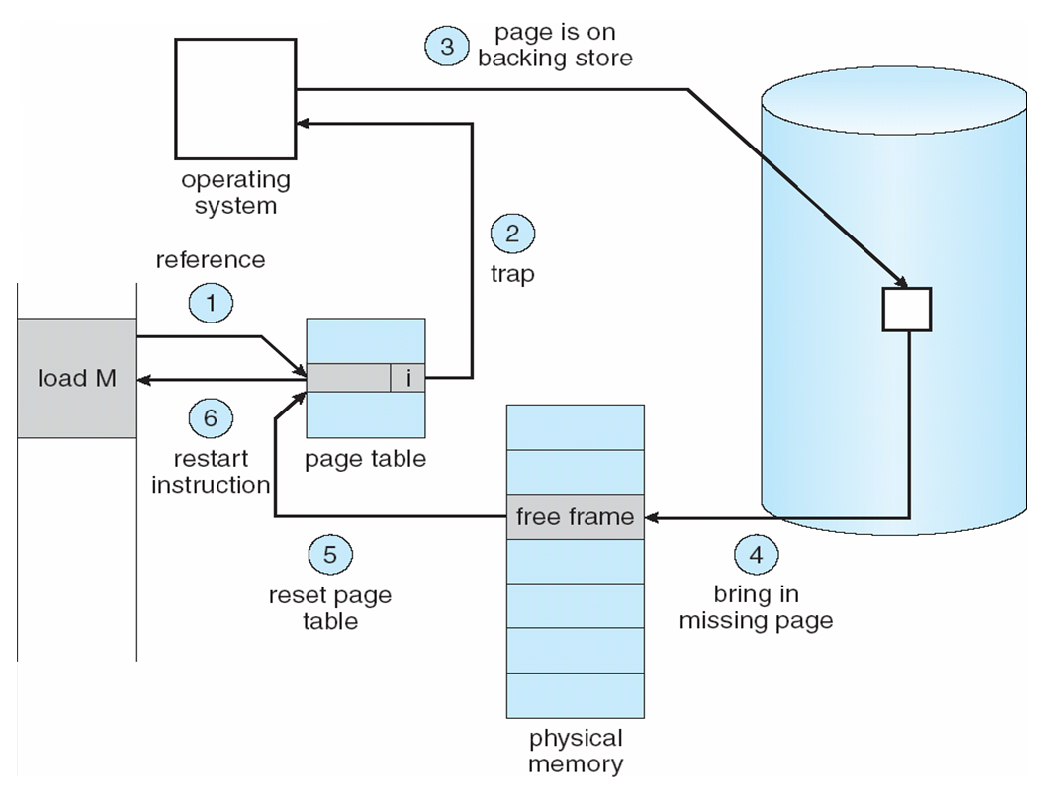
\includegraphics[height=2.7in]{figs/pagefault}}
\itms{
  \item Use disk to simulate larger virtual than physical mem
}
\end{frame}

\pgfmathsetseed{2}
\def\refpointsA{}
\def\refpointsB{}
\foreach \x in {0,.05,...,9.8} {
    \pgfmathsetmacro{\phase}{mod(floor(\x), 3) == 2}
    \ifcase\phase
      \pgfmathparse{max(0,.1+.15*rand)}
      \xdef\refpointsA{\refpointsA (\x, \pgfmathresult)}
    \else
      \pgfmathparse{2+rand}
      \xdef\refpointsB{\refpointsB (\x, \pgfmathresult)}
    \fi}

\begin{frame}{Working set model}\relax
\begin{tikzpicture}
\begin{scope}[thick, ycomb, few-blue]
\draw[only=<2>{few-red}] plot coordinates{\refpointsB};
\draw[only=<3>{few-red}] plot coordinates{\refpointsA};
\end{scope}
\draw[very thick, <->] (0, 3) --
    node[midway, rotate=90, above] {\# of accesses} (0,0)
    -- node[midway, below] {virtual address} (10,0);
\path[very thick, few-red, alt=<2>{opacity=.8}{opacity=0},
    ellipse, inner ysep=-.25cm]
  foreach \x in {2,5,8} {
      node[draw,fit={(\x,0) (\x+1,3)}] {} };
\path[very thick, few-red, alt=<3>{opacity=.8}{opacity=0}, ellipse]
  foreach \x in {0,3,6} {
      node[draw,fit={(\x,0) (\x+2,.25)}, inner xsep=-.2cm] {}
  }
  node[draw,fit={(9,0) (9.8,.25)}, inner xsep=-.05cm] {};
\end{tikzpicture}
\itms{
  \item Disk much, much slower than memory
  \ittms{
    \item Goal:  run at memory speed, not disk speed
  }
  \item 80/20 rule:  20\% of memory gets 80\% of memory accesses
  \ittms{
    \item<redbullet@2> Keep the hot 20\% in memory
    \item<redbullet@3> Keep the cold 80\% on disk
  }
  %\item Challenge:  how to identify the hot 20\%?
}
\end{frame}

\begin{slide}{Paging challenges}
\itms{
  \item How to resume a process after a fault?
\ittms{
\item Need to save state and resume
\item Process might have been in the middle of an instruction!
}
  \item What to fetch from disk?
\ittms{
\item Just needed page or more?
}
  \item What to eject?
\ittms{
  \item How to allocate physical pages amongst processes?
  \item Which of a particular process's pages to keep in memory?
}
}
\end{slide}

\begin{slide}{Re-starting instructions}
\itms{
  \item Hardware provides kernel with information about page fault
  \ittms{
    \item Faulting virtual address (In \texttt{\%c0\_vaddr} reg on MIPS)
    \item Address of instruction that caused fault (\texttt{\%c0\_epc} reg)
    \item Was the access a read or write?  Was it an instruction
  fetch? \\
      Was it caused by user access to kernel-only memory?
  }
  \item Hardware must allow resuming after a fault
  \item Idempotent instructions are easy
  \ittms{
    \item E.g., simple load or store instruction can be restarted
    \item Just re-execute any instruction that only accesses one
  address
  }
}
\end{slide}

\begin{slide}{What to fetch}
\itms{
  \item Bring in page that caused page fault
  \item Pre-fetch surrounding pages?
  \ittms{
    \item Reading two disk blocks approximately as fast as reading one
    \item As long as no track/head switch, seek time dominates
    \item If application exhibits spacial locality, then big win to
  store and read multiple contiguous pages
  }
  \item Also pre-zero unused pages in idle loop
  \ittms{
    \item Need 0-filled pages for stack, heap, anonymously mmapped memory
    \item Zeroing them only on demand is slower
    \item Hence, many OSes zero freed pages while CPU is idle
  }
}
\end{slide}

\begin{slide}{Selecting physical pages}
\itms{
  \item May need to eject some pages
  \ittms{
    \item More on eviction policy in two slides
  }
  \item May also have a choice of physical pages
  \item Direct-mapped physical caches
  \ittms{
    \item Virtual $\to$ Physical mapping can affect performance
    \item In old days: Physical address $A$ conflicts with $kC+A$ \\
      (where $k$ is any integer, $C$ is cache size)
    \item Applications can conflict with each other or themselves
    \item Scientific applications benefit if consecutive virtual pages
          do not conflict in the cache
    \item Many other applications do better with random mapping
    \item These days: CPUs more sophisticated than $kC+A$
  }
}
\end{slide}

\begin{slide}{Superpages}
\itms{
  \item How should OS make use of ``large'' mappings
  \ittms{
    \item x86 has 2/4MB pages that might be useful
    \item Alpha has even more choices: 8KB, 64KB, 512KB, 4MB
  }
  \item Sometimes more pages in L2 cache than TLB entries
  \ittms{
    \item Don't want costly TLB misses going to main memory
  }
  \item Or have two-level TLBs
  \ittms{
    \item Want to maximize hit rate in faster L1 TLB
  }
  \item OS can transparently support superpages
    \href{http://www.usenix.org/events/osdi02/tech/full_papers/navarro/navarro.pdf}{[Navarro]}
  \ittms{
    \item ``Reserve'' appropriate physical pages if possible
    \item Promote contiguous pages to superpages
    \item Does complicate evicting (esp.\ dirty pages) -- demote
  }
}
\end{slide}

\section{Eviction policies}

\begin{frame}
\frametitle{Straw man:  FIFO eviction}
\itms{
  \item Evict oldest fetched page in system
  \item Example---reference string 1, 2, 3, 4, 1, 2, 5, 1, 2, 3, 4, 5
  \item 3 physical pages: 9 page faults
\begin{overlayarea}{\textwidth}{32mm}
\only<1>{\item[] 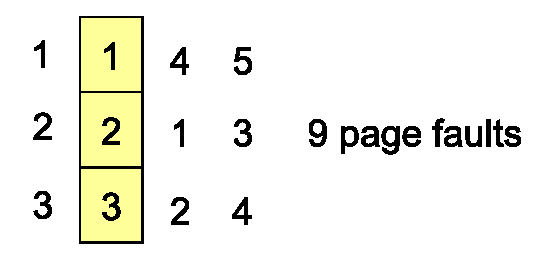
\includegraphics[width=2in]{figs/fifo1}}
\only<2>{
  \item \bfseries 4 physical pages: 10 page faults \\[1ex]
	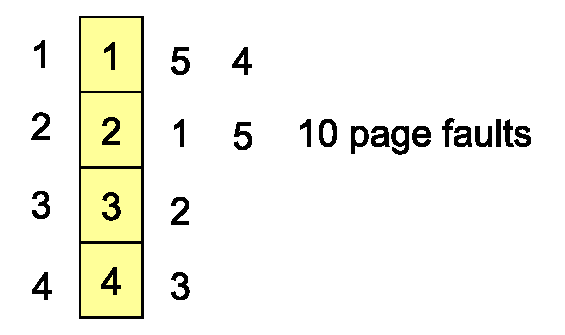
\includegraphics[width=2in]{figs/fifo2}
}
\end{overlayarea}
}
\end{frame}

\begin{slide}{Belady's Anomaly}
\centerline{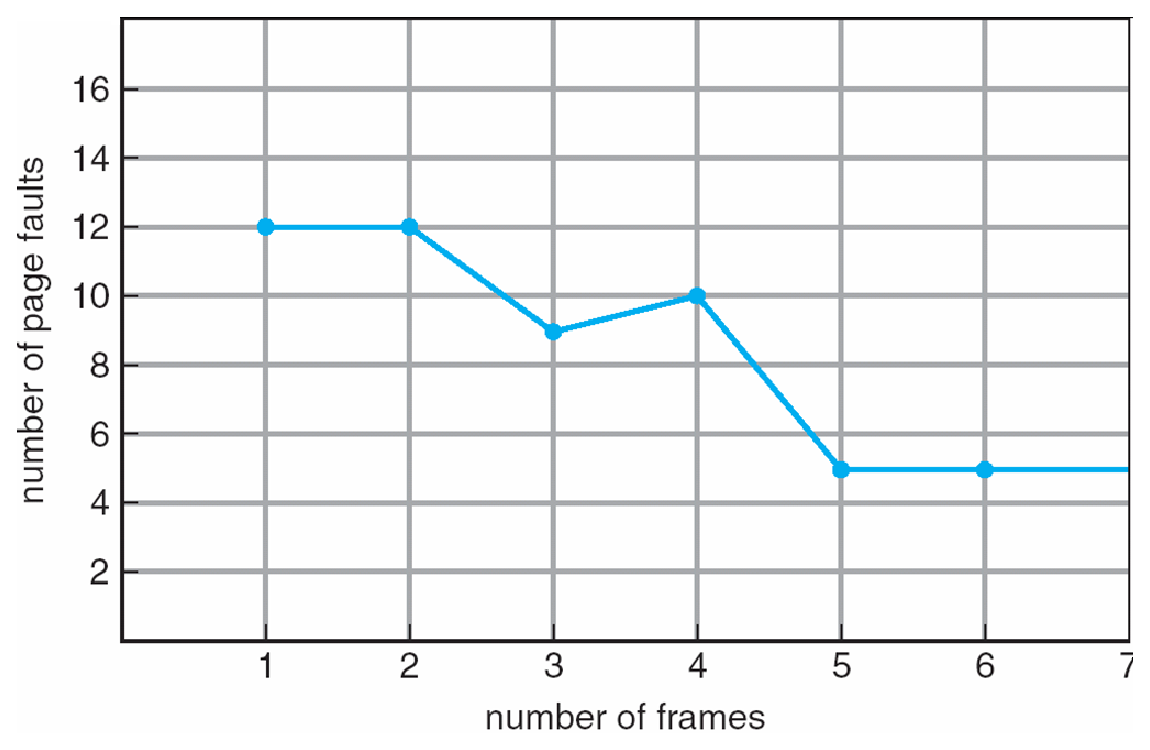
\includegraphics[width=3.8in]{figs/belady}}

\medskip

\itms{
  \item More physical memory doesn't always mean fewer faults
}
\end{slide}

\begin{frame}
\frametitle{Optimal page replacement}
\itms{
\item What is optimal (if you knew the future)?
\pause
\ittms{
  \item Replace page that will not be used for longest period of time
}
\item  Example---reference string 1, 2, 3, 4, 1, 2, 5, 1, 2, 3, 4, 5
\item With 4 physical pages: \\[1ex]
	\centerline{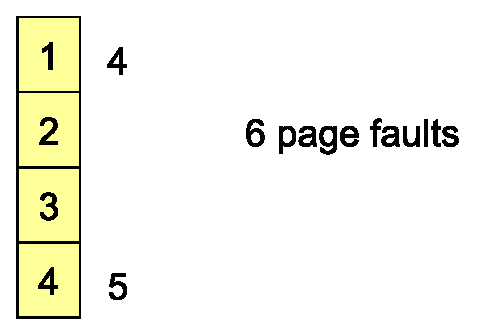
\includegraphics[width=2in]{figs/optimal}}
}
\end{frame}

\begin{slide}{LRU page replacement}
\itms{
  \item Approximate optimal with \emph{least recently used}
  \ittms{
    \item Because past often predicts the future
  }
  \item  Example---reference string 1, 2, 3, 4, 1, 2, 5, 1, 2, 3, 4, 5
  \item With 4 physical pages: 8 page faults \\[1ex]
    \centerline{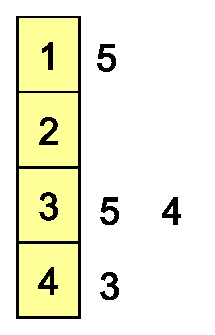
\includegraphics[height=1.3in]{figs/lru}}
  \item Problem 1:  Can be pessimal -- example?
\onslide<2>{
  \ittms{
      \item Looping over memory (then want MRU eviction)
  }
}
  \item Problem 2:  How to implement?
}
\end{slide}

\begin{slide}{Straw man LRU implementations}
\itms{
\item Stamp PTEs with timer value
\ittms{
  \item E.g., CPU has cycle counter
  \item Automatically writes value to PTE on each page access
  \item Scan page table to find oldest counter value = LRU page
  \item Problem: Would double memory traffic!
}
\item Keep doubly-linked list of pages
\ittms{
  \item On access remove page, place at tail of list
  \item Problem:  again, very expensive
}
\item What to do?
\ittms{
  \item Just approximate LRU, don't try to do it exactly
}
}
\end{slide}

\def\acolors{{"few-green-light", "few-red-light"}}
\tikzset{
    clocknode/.code={%
        \pgfmathsetmacro\a{0 != #1}%
        \pgfmathsetmacro\c{\acolors[\a]}%
        \pgfkeysalso{anchor=center, node contents={$A=\a$}, circle, fill=\c}},
    altclocknode/.code args={<#1>}{%
        \alt<#1>{\def\a{1}}{\def\a{0}}%
        \pgfkeysalso{clocknode=\a}},
}
\def\hand<#1>#2{%
    \draw[visible=<#1>,very thick, ->, shorten >=1pt] (0,0)
    node[pos=0, circle, fill] {} -- (#2);}

\begin{frame}
\frametitle{Clock algorithm}
\itms{
  \item Use accessed bit supported by most hardware
  \ittms{
    \item E.g., Pentium will write 1 to A bit in PTE on first access
    \item Software managed TLBs like MIPS can do the same
  }
}
\begin{columns}[T,onlytextwidth]
\column{65mm}
\itms{
  \item Do FIFO but skip accessed pages
  \item Keep pages in circular \rlap{FIFO list}
  \item Scan:
  \ittms{
    \item page's A bit = 1, set to 0 \& skip
    \item else if A = 0, evict
  }
  \item A.k.a. second-chance \rlap{replacement}
}
\column{50mm}
\pgfmathsetseed{2}
\begin{tikzpicture}[node font=\footnotesize, inner sep=1pt]
\foreach \x in {0,1,2,6,7,...,11}
    \node[clocknode={random(0,1)}, at={(\x*30:1.9cm)}, name=n\x];
\node[clocknode=0, at={(5*30:1.9cm)}, name=n5];
\node[altclocknode=<1>, at={(4*30:1.9cm)}, name=n4];
\node[clocknode=0, at={(3*30:1.9cm)}, name=n3];
\draw[very thick, ->] (150:2.5cm) arc[start angle=150, end angle=90,
    radius=2.5cm];
\hand<1>{n5}
\hand<2>{n4}
\hand<3>{n3}
\node[opacity=.5, visible=<3>, at=(n3.center), draw=few-red-bright,
    cross out, line width=4pt, minimum size=2em, line cap=round]
    {};
\end{tikzpicture}
\end{columns}
\end{frame}

\begin{frame}
\frametitle{Clock algorithm (continued)}
\vspace{-0.5em}
\begin{columns}[c,onlytextwidth]
\column{73mm}
\itms{
  \item Large memory may be a problem
  \ittms{
    \item Most pages referenced in long interval
  }
  \item Add a second clock hand
  \ittms{
    \item Two hands move in lockstep
    \item Leading hand clears A bits
    \item Trailing hand evicts pages with A=0
  }
}
\column{46mm}
%% \pgfmathsetseed{2}
%% \begin{tikzpicture}[node font=\footnotesize, inner sep=1pt]
%% \foreach \x in {0,...,11} {
%%   \pgfmathsetmacro\a{random(0,1)}
%%   \pgfmathsetmacro\c{\acolors[\a]}
%%   \node[anchor=center, fill=\c, circle]
%%     at (\x*30:1.9cm) (n\x) {$A=\a$};
%% }
%% \node[anchor=center, visible=<1>, at=(n1.center), fill=few-red-light,
%%     circle] {$A=1$};
%% %\node[visible=<2>,
%% %    at=(n4.center), anchor=center, fill=few-green-light, circle]
%% %    {$A=0$};
%% \node[opacity=.5, visible=<2>, at=(n3.center), draw=few-red-bright,
%%     cross out, line width=4pt, minimum size=2em, line cap=round]
%%     {};
%% \draw[visible=<1>, very thick, ->, shorten >=1pt] (0,0) node[pos=0, circle, fill] {} -- (n4);
%% \draw[visible=<1>, very thick, ->, shorten >=1pt] (0,0) node[pos=0, circle, fill] {} -- (n1);
%% \draw[visible=<2>, very thick, ->, shorten >=1pt] (0,0) node[pos=0, circle, fill] {} -- (n3);
%% \draw[visible=<2>, very thick, ->, shorten >=1pt] (0,0) node[pos=0,
%%     circle, fill] {} -- (n0);
%% \draw[very thick, ->] (150:2.5cm) arc[start angle=150, end angle=90,
%%     radius=2.5cm];
%% \end{tikzpicture}
\begin{tikzpicture}[node font=\footnotesize, inner sep=1pt]
\pgfmathsetseed{2}
\foreach \x in {0,3,5,6,...,11}
    \node[clocknode={random(0,1)}, at={(\x*30:1.9cm)}, name=n\x];
\node[clocknode=0, at={(2*30:1.9cm)}, name=n2];
\node[altclocknode=<1>, at={(1*30:1.9cm)}, name=n1];
\node[clocknode=4, at={(4*30:1.9cm)}, name=n4];
\draw[very thick, ->] (150:2.5cm) arc[start angle=150, end angle=90,
    radius=2.5cm];
\hand<1>{n5}
\hand<1>{n2}
\hand<2>{n4}
\hand<2>{n1}
\hand<3>{n3}
\hand<3>{n0}
\node[opacity=.5, visible=<3>, at=(n3.center), draw=few-red-bright,
    cross out, line width=4pt, minimum size=2em, line cap=round]
    {};
\end{tikzpicture}
\end{columns}
\vspace*{-1em}
\itms{
  \item Can also take advantage of hardware Dirty bit
  \ittms{
    \item Each page can be (Unaccessed, Clean), (Unaccessed, Dirty),
      (Accessed, Clean), or (Accessed, Dirty)
    \item Consider clean pages for eviction before dirty
  }
  \item Or use $n$-bit accessed \emph{count} instead just $A$ bit
  \ittms{
    \item On sweep:
  $\mathit{count}=(A<\!\!<(n-1))\>|\> (\mathit{count}>\!\!>1)$ft
    \item Evict page with lowest \emph{count}
  }
}
\end{frame}

\begin{slide}{Other replacement algorithms}
\itms{
  \item Random eviction
  \ittms{
    \item Simple to implement
    \item Not overly horrible (avoids Belady \& pathological cases)
    \item Used in hypervisors to avoid double swap \cref{readings/esxrm.pdf}{[Waldspurger]}
  }
  \item \emph{LFU} (least frequently used) eviction
%  \ittms{
%   \item Instead of just A bit, count \# times each page accessed
%   \item Least frequently accessed must not be very useful \\
%         (or maybe was just brought in and is about to be used)
%   \item Decay usage counts over time (for pages that fall out of
%  usage)
%  }
  \item \emph{MFU} (most frequently used) algorithm
%  \ittms{
%    \item Because page with the smallest count was probably just
%      brought in and has yet to be used
%  }
  \item Neither LFU nor MFU used very commonly
  \item Workload specific policies: Databases
}
\end{slide}

\begin{slide}{Na\"\i ve paging}
\centerline{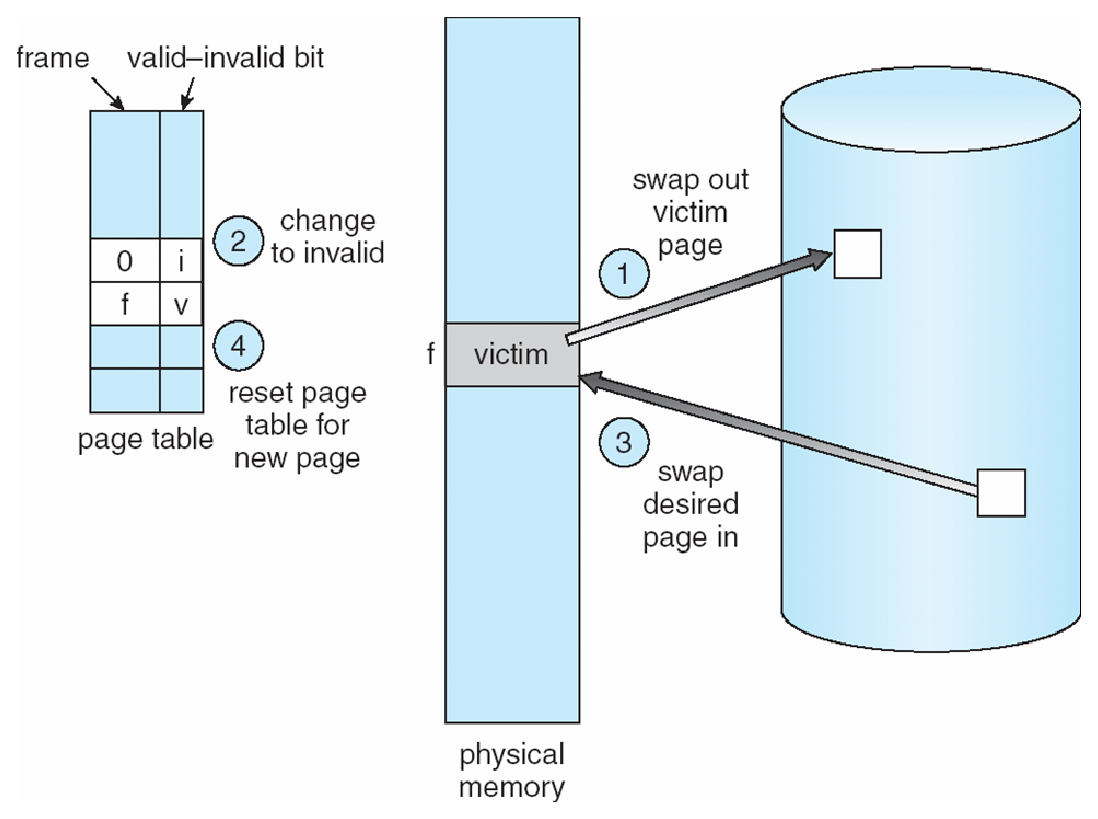
\includegraphics[height=2.7in]{figs/replacement}}
\itms{
  \item Na\"\i ve page replacement: 2 disk I/Os per page fault
}
\end{slide}

\begin{slide}{Page buffering}
\itms{
  \item Idea: reduce \# of I/Os on the critical path
  \item Keep pool of free page frames
  \ittms{
    \item On fault, still select victim page to evict
    \item But read fetched page into already free page
    \item Can resume execution while writing out victim page
    \item Then add victim page to free pool 
  }
  \item Can also yank pages back from free pool
  \ittms{
    \item Contains only clean pages, but may still have data
    \item If page fault on page still in free pool, recycle
  }
}
\end{slide}

\begin{frame}{Page allocation}
\itms{
  \item Allocation can be \emph{global} or \emph{local}
  \item Global allocation doesn't consider page ownership
  \ittms{
    \item E.g., with LRU, evict least recently used page of any proc
    \item Works well if $P_1$ needs 20\% of memory and $P_2$ needs 70\%:
      \\[2pt]
\begin{tikzpicture}[outer xsep=0, node distance=0,
        start chain=going right, minimum height=3ex,
    every node/.style={on chain, draw}, semithick]
\node[colornode=green, minimum width=1cm] {$P_1$};
\node[minimum width=.5cm] {};
\node[colornode=orange, minimum width=3.5cm] {$P_2$};
\end{tikzpicture}
    \item Doesn't protect you from memory pigs \\
      (imagine $P_2$ keeps looping through array that is size of mem)
  }
  \item Local allocation isolates processes (or users)
  \ittms{
    \item Separately determine how much memory each process should have
    \item Then use LRU/clock/etc.\ to determine which pages to evict
  within each process
  }
}
\end{frame}

\section{Thrashing}

\begin{slide}{Thrashing}
\begin{block}{}
{\em Thrashing} is when an application is in a constantly swapping pages in and 
	out preventing the application from making forward progress at any 
	reasonable rate.
\end{block}
\itms{
  \item Processes require more memory than system has
  \ittms{
    \item Each time one page is brought in, another page, whose
      contents will soon be referenced, is thrown out
    \item Processes will spend all of their time blocked, waiting for
      pages to be fetched from disk
    \item I/O devs at 100\% utilization but system not getting much
      useful work done 
  }
  \item What we wanted: virtual memory the size of disk with access
    time the speed of physical memory
  \item What we got: memory with access time of disk
}
\end{slide}

\begin{frame}{Reasons for thrashing}
\itms{
  \item Access pattern has no temporal locality (past $\ne$ future)
  \begin{itemize}
    \item[]
\begin{tikzpicture}
\begin{scope}[very thick, few-blue]
%\foreach \x in {0, 0.067, ..., 4.85} \draw (\x,0) -- (\x, 0.7 + 0.1*rnd);
\draw[ycomb, domain={0:4.8}, samples=64] plot (\x, 0.7 + 0.1*rand);
\end{scope}
\draw[very thick, <->] (0, 1) -- (0,0) -- (5,0);        
\end{tikzpicture}
      \quad (80/20 rule has broken down)
  \end{itemize}
\item Hot memory does not fit in physical memory
  \begin{itemize}
    \item[]
\begin{tikzpicture}
\node[colornode=gray-light] (memory) {\strut memory};
\node[colornode=green, above=0pt of memory, minimum width=3cm]
     (p1) {\strut};
\begin{scope}[on background layer]
    \filldraw[colornode=green-light] (p1.south west)
    rectangle ([xshift=5cm] p1.north east) node[midway] {$P_1$};
\end{scope}
\end{tikzpicture}
  \end{itemize}
\item Each process fits individually, but too many for system
\ittms{
    \item[]
\def\proccolors{{"green", "orange", "blue", "pink", "brown", "purple", "red"}}
\begin{tikzpicture}
\foreach \x in {1,...,16} {
   \pgfmathsetmacro\c{\proccolors[mod(\x-1,7)]}
   \node[draw,colornode=\c, minimum width=2em, anchor=south]
   at (0.5*\x, {0.2*mod(\x,2)}) {$P_{\x}$};
}
\node[colornode=gray-light, anchor=north, minimum width=4cm]
     at (current bounding box.south |- 0,0)
     {\strut memory};
\end{tikzpicture}
    \item At least this case is possible to address
}
}
\end{frame}

% \begin{slide}{Multiprogramming \& Thrashing}
% 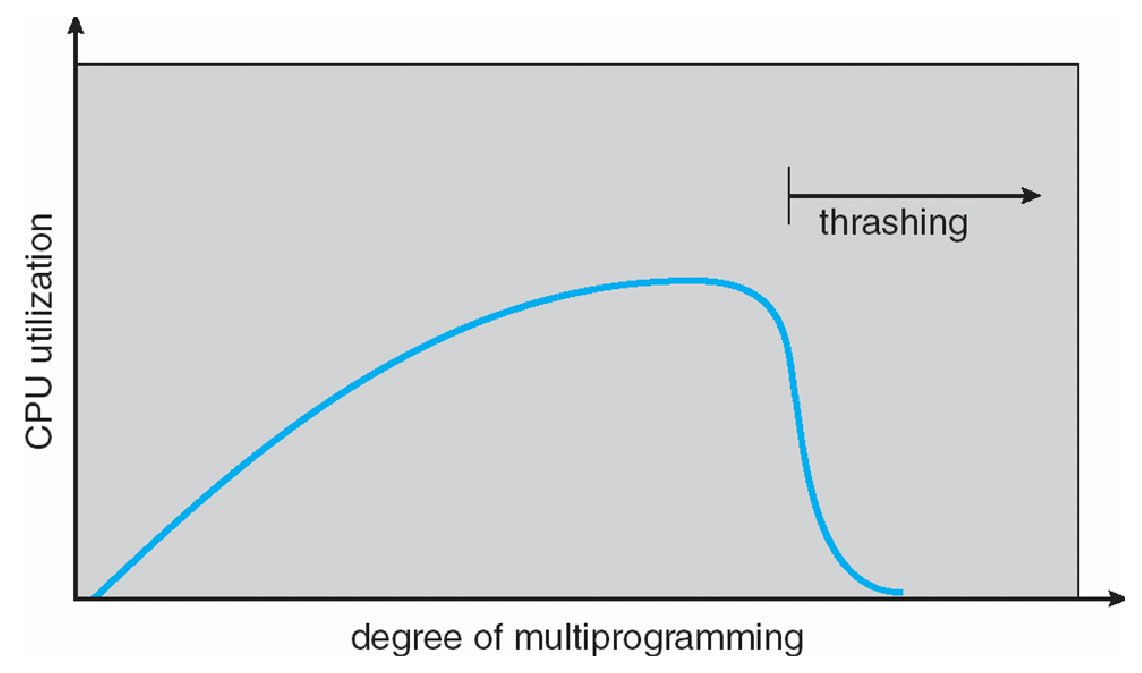
\includegraphics[width=112mm]{figs/thrashing}

% \medskip

% \itms{
%   \item Must shed load when thrashing
% }
% \end{slide}

\begin{slide}{Dealing with thrashing}
\itms{
\item Approach 1:  working set 
\ittms{
  \item Thrashing viewed from a caching perspective: given locality of reference, how big a cache does the process need?
  \item Or: how much memory does the process need in order to make reasonable progress (its working set)?
  \item Only run processes whose memory requirements can be satisfied
}
\item Approach 2: page fault frequency
\ittms{
  \item Thrashing viewed as poor ratio of fetch to work
  \item PFF = page faults / instructions executed 
  \item If PFF rises above threshold, process needs more memory. \\
  Not enough memory on the system? Swap out.
  \item If PFF sinks below threshold, memory can be taken away 
}
}
\end{slide}

\begin{frame}{Working sets}
\pgfmathsetseed{2}
\begin{tikzpicture}
\draw[few-blue, very thick, smooth, domain={0:9.8}, name path=graph] plot
(\x, { \x < 1.0 ? \x *rnd :
    (mod(floor(\x) + 1, 3) ?
    0.5*floor(mod(\x,9)/3) + 1+0.1*rand
    : 3.5+0.2*rand ) });
\draw[very thick,<->] (0,4) -- node[rotate=90, above]
     {working set size} (0,0) -- node[below] {time} (10,0);
\begin{scope}[on background layer={thick, few-gray}]
\foreach \x in {1.7, 3.2, 4.9, 6.1, 7.8, 9.4} {
    \path[name path=vert] (\x,0) -- (\x,4);
    \draw[name intersections={of=graph and vert}, dashed]
    (\x, 0) -- (intersection-1);
}
\end{scope}
\tikzset{trans/.style={thick, few-gray, ->, opacity=.8}}
\node[trans,opacity=1] at (4.05,4) (transitions) {Transitions};
\draw[trans] (transitions) -- (2.5,3);
\draw[trans] (transitions) -- (5.5,3);
\draw[trans] (transitions.0) to[out=0, in=135] (8.5,3);
\end{tikzpicture}
\bigskip
\itms{
  \item Working set changes across phases
  \ittms{
    \item Baloons during phase transitions
  }
}
\end{frame}

% \begin{slide}{Calculating the working set}
% \itms{
%   \item Working set:  all pages process will access in next $T$ time
%   \ittms{
%     \item Can't calculate without predicting future
%   }
%   \item Approximate by assuming past predicts future
%   \ittms{
%     \item So working set $\approx$ pages accessed in last $T$ time
%   }
%   \item Keep idle time for each page
%   \item Periodically scan all resident pages in system
%   \ittms{
%     \item \textbf{A} bit set?  Clear it and clear the page's idle time
%     \item \textbf{A} bit clear?  Add CPU consumed since last scan to idle time
%     \item Working set is pages with idle time $<T$
%   }
% } 
% \end{slide}

% \begin{slide}{Two-level scheduler}
% \itms{
%   \item Divide processes into \emph{active} \& \emph{inactive}
%   \ittms{
%     \item Active -- means working set resident in memory
%     \item Inactive -- working set intentionally not loaded
%   }
%   \item Balance set: union of all active working sets
%   \ittms{
%     \item Must keep balance set smaller than physical memory
%   }
%   \item Use long-term scheduler [recall from lecture 4]
%   \ittms{
%     \item Moves procs active $\to$ inactive until balance set
% 	  small \rlap{enough}
%     \item Periodically allows inactive to become active
%     \item As working set changes, must update balance set
%   }
%   \item Complications
%   \ittms{
%     \item How to chose idle time threshold $T$?
%     \item How to pick processes for active set
%     \item How to count shared memory (e.g., libc.so)
%   }
% }
% \end{slide}

% OLDSPLIT

\begin{slide}{Virtual memory goals}
\centerline{\includegraphics[width=112mm]{vmhilevel}}
\vspace{-2em}
\itms{
  \item Give each program its own ``virtual'' address space
  \ittms{
    \item At run time, Memory-Management Unit relocates each load,
      store to actual memory\ldots\ App doesn't see physical memory
  }
  \item Enforces protection
  \item Allows programs to see more memory than exists
}
\end{slide}

\begin{frame}{Paging}
\centerline{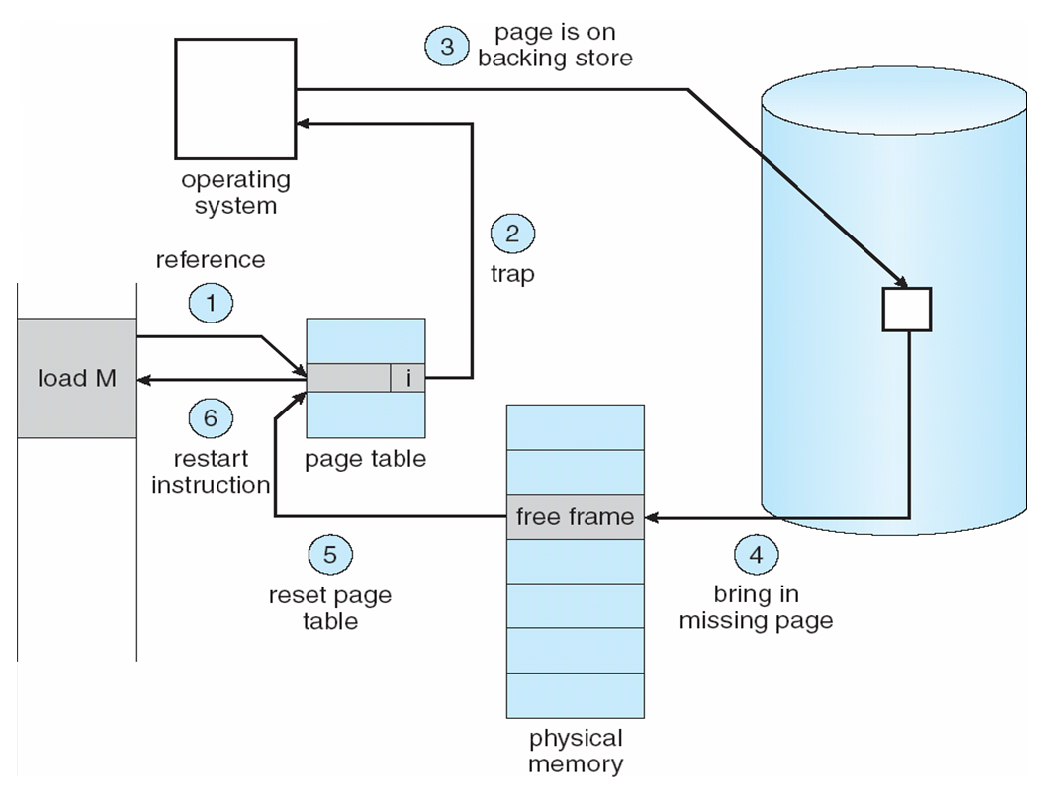
\includegraphics[height=2.7in]{figs/pagefault}}
\itms{
  \item Use disk to simulate larger virtual than physical mem
}
\end{frame}

% \section{OS/161 Virtual Memory}

% \begin{slide}{MIPS Memory Layout}
% \begin{bytefield}{16}
% 	\begin{rightwordgroup}{Kernel Memory}
% 	\memsection{FFFF FFFF}{C000 0000}{4}{kseg2: Paged Kernel}\\
% 	\memsection{BFFF FFFF}{A000 0000}{2}{kseg1: Phys. Uncached}\\
% 	\memsection{9FFF FFFF}{8000 0000}{2}{kseg0: Phys. Cached}
% 	\end{rightwordgroup}\\
% 	\begin{rightwordgroup}{User Memory}
% 	\memsection{7FFF FFFF}{0000 0000}{8}{kuseg: Paged User\\{\tt dumbvm}}
% 	\end{rightwordgroup}
% \end{bytefield}
% \end{slide}

% \begin{slide}{OS/161 dumbvm Address Translation}
% \begin{ccode}
% struct addrspace {
%   vaddr_t as_vbase1; /* Segment 1 */
%   paddr_t as_pbase1;
%   size_t as_npages1;
%   vaddr_t as_vbase2; /* Segment 2 */
%   paddr_t as_pbase2;
%   size_t as_npages2;
%   paddr_t as_stackpbase; /* Stack Base */
% };
% \end{ccode}
% \itms{
%   \item Implements segments with a TLB!
%   \item Three segments code, data, and a fixed stack
%   \item Virtual base (vbase), Physical base (pbase), and Number of pages 
% 	  (npages)
%   \item Stack has a physical base address
% }
% \end{slide}

% \begin{slide}{OS/161 dumbvm Segments}
% \itms{
%   \item $vbase$: Virtual Base Address
%   \item $vtop = vbase + npages * PAGE\_SIZE$: Virtual Top Address
%   \item Segment maps memory between vbase and vtop
%   \vspace{1em}
%   \item $pbase$: Physical Base Address
%   \item $paddr = faddr - vbase + pbase$ : Convert Physical to Virtual
%   \vspace{1em}
%   \item Stack is always 12 pages in size
%   \item Grows down from the top of memory
%   \vspace{1em}
%   \item Looks a like like the original UNIX releases in the 80s
%   \item Assignment 3 you will replace this with a RADIX tree (similar to x86)
% }
% \end{slide}

% \begin{slide}{OS/161 Memory Layout: user/testbin/sort}
% \itms{
%   \vspace{-1em}
%   \item Example: \texttt{vbase1=0x400000}, \texttt{npages1=0x2}, 
% 	  \texttt{pbase1=XXXXXXXX},\\
% 	  \texttt{vbase2=0x10000000}, \texttt{npages2=0x12}, 
% 	  \texttt{pbase2=YYYYYYYY},\\
% 	  \texttt{stackpbase=ZZZZZZZZ}
% }
% \begin{bytefield}{15}
% 	\memsection{7FFF FFFF}{7FF4 0000}{2}{Stack}\\
% 	\memsection{}{}{6}{}\\
% 	\memsection{1012 00B0}{1000 0000}{2}{Data}\\
% 	\memsection{}{}{2}{}\\
% 	\memsection{0040 1A0C}{0040 0000}{2}{Text + R/O Data}\\
% 	\memsection{}{}{1}{}\\
% \end{bytefield}
% \end{slide}

% \begin{slide}{OS/161 dumbvm Translation Logic}
% \begin{ccode}
% // USERSTACK=0x8000_0000, DUMBVM_STACKPAGES=12
% // PAGE_SIZE=4K
% vbase1 = as->as_vbase1;
% vtop1 = vbase1 + as->as_npages1 * PAGE_SIZE;
% vbase2 = as->as_vbase2;
% vtop2 = vbase2 + as->as_npages2 * PAGE_SIZE;
% stackbase = USERSTACK - DUMBVM_STACKPAGES * PAGE_SIZE;
% stacktop = USERSTACK;

% if (faultaddr >= vbase1 && faultaddr < vtop1) {
%   paddr = (faultaddr - vbase1) + as->as_pbase1;
% } else if (faultaddr >= vbase2 && faultaddr < vtop2) {
%   paddr = (faultaddr - vbase2) + as->as_pbase2;
% } else if (faultaddr >= stackbase && faultaddr < stacktop) {
%   paddr = (faultaddr - stackbase) + as->as_stackpbase;
% } else {
%   return EFAULT;
% }
% \end{ccode}
% \end{slide}

% \begin{slide}{OS/161 Details}
% \itms{
%   \item TLB fault exception calls:
%   \ittms{
%     \item \texttt{common\_exception} pushes trap frame
%     \item \texttt{mips\_trap()} determines trap cause and calls 
% 	    \texttt{vm\_fault()}
%     \item \texttt{vm\_fault()} computes physical address from faulting address
%     \item Calls \texttt{tlb\_write()} to update the TLB and returns
%   }
%   \vspace{1em}
%   \item Address Spaces APIs
%   \ittms{
%     \item \texttt{as\_define\_region()} creates a segment (2 max)
%     \item \texttt{as\_activate()} invalidates the TLB
%     \item \texttt{as\_copy()} duplicates the entire process
%   }
% }
% \end{slide}

% \begin{slide}{OS/161 and ELF: \texttt{readelf}}
% \vspace{-1em}
% \lstset{basicstyle=\small\ttfamily\openup-.17\baselineskip,columns=flexible}
% \begin{lstlisting}
% ELF Header:
%   Magic:   7f 45 4c 46 02 01 01 09 00 00 00 00 00 00 00 00 
%   Class:                             ELF64
%   Data:                              2's complement, little endian
%   Version:                           1 (current)
%   OS/ABI:                            FreeBSD
%   ABI Version:                       0
%   Type:                              EXEC (Executable file)
%   Machine:                           Advanced Micro Devices x86-64
%   Version:                           0x1
%   Entry point address:               0x203000
%   Start of program headers:          64 (bytes into file)
%   Start of section headers:          38416 (bytes into file)
%   Flags:                             0
%   Size of this header:               64 (bytes)
%   Size of program headers:           56 (bytes)
%   Number of program headers:         10
%   Size of section headers:           64 (bytes)
%   Number of section headers:         29
%   Section header string table index: 28
% \end{lstlisting}
% \itms{
%   \item Describes the binary and starting point (entry point)
% }
% \end{slide}

% \begin{slide}{OS/161 and ELF: \texttt{readelf}}
% \vspace{-1em}
% \lstset{basicstyle=\small\ttfamily\openup-.17\baselineskip,columns=flexible}
% \begin{lstlisting}
% Program Headers:
%   Type           Offset             VirtAddr           PhysAddr
%                  FileSiz            MemSiz              Flg    Align
%   PHDR           0x00000000000040 0x00000000200040 0x00000000200040
%                  0x00000000000230 0x00000000000230  R      0x8
%   INTERP         0x00000000000270 0x00000000200270 0x00000000200270
%                  0x00000000000015 0x00000000000015  R      0x1
%       [Requesting program interpreter: /libexec/ld-elf.so.1]
%   LOAD           0x00000000000000 0x00000000200000 0x00000000200000
%                  0x00000000002bd8 0x00000000002bd8  R      0x1000
%   LOAD           0x00000000003000 0x00000000203000 0x00000000203000
%                  0x00000000004b50 0x00000000004b50  R E    0x1000
%   LOAD           0x00000000008000 0x00000000208000 0x00000000208000
%                  0x000000000011a0 0x0000000000229c  RW     0x1000
%   ...
% \end{lstlisting}
% \itms{
%   \item Program Headers are instructions for the OS
%   \item \texttt{INTERP} is the dynamic linker (more in a later class)
%   \item \texttt{LOAD} is a single segment for the OS to load
%   \item Shown is /bin/ls from FreeBSD and it has more than two segments
% }
% \end{slide}

\section{User-level API}

\begin{frame}{Recall typical virtual address space}
\relax{\centering
\begin{tikzpicture}[
        start chain=going below, node distance=0, outer ysep=0,
    align=center, thick]
\begin{scope}[every node/.style={on chain}, text width=5cm,
        minimum height=3ex]
\node[colornode=red, text width={5cm+\pgflinewidth}] {kernel};
\tikzset{every node/.append style={thin, draw, outer sep=0pt}}
\node[colornode=green] (stack) {stack};
\node[colornode=green, below=1.5cm of stack] (heap) {\smash[b]\strut heap};
\node[colornode=green] {uninitialized data (bss)};
\node[colornode=blue] {initialized data};
\node[colornode=gray-light] {read-only data};
\node[colornode=gray-light] (text) {code (text)};
\end{scope}
\draw[->] (stack.south) -- +(0, -.5);
\draw[->] (heap.north) -- +(0, .5);
\draw[alert-color,<-,shorten <=2pt]
  (heap.north east) -- +(1.5,0) node[right] {breakpoint};
\draw[ultra thick, few-red-bright] (heap.north west) -- (heap.north east);
\node[inner sep=0, draw, fit={(stack) (text)}] {};
\end{tikzpicture}\\}
\smallskip
\itms{
  \item Dynamically allocated memory goes in heap
%  \ittms{
%    \item Typically right above BSS (uninitialized data) section
%  }
  \item Top of heap called \emph{breakpoint}
  \ittms{
    \item Addresses between breakpoint and stack all invalid
  }
}
\end{frame}

\begin{slide}{Early VM system calls}
\itms{
  \item OS keeps ``Breakpoint'' -- top of heap
  \ittms{
    \item Memory regions between breakpoint \& stack fault on access
  }
  \item \texttt{char *brk (const char *addr);}
  \ittms{
    \item Set and return new value of breakpoint
  }
  \item \texttt{char *sbrk (int incr);}
  \ittms{
    \item Increment value of the breakpoint \& return old value
  }
  \item Can implement \texttt{malloc} in terms of \texttt{sbrk}
  \ittms{
    \item But hard to ``give back'' physical memory to system
  }
}
\end{slide}

\begin{frame}{Memory mapped files}
\relax{\centering
\begin{tikzpicture}[
        start chain=going below, node distance=0, outer ysep=0,
    align=center, thick]
\begin{scope}[every node/.style={on chain}, text width=5cm,
        minimum height=3ex]
\node[colornode=red, text width={5cm+\pgflinewidth}] {kernel};
\tikzset{every node/.append style={thin, draw, outer sep=0pt}}
\node[colornode=green] (stack) {stack};
\node[colornode=green, below=1.5cm of stack] (heap) {\smash[b]\strut heap};
\node[colornode=green] {uninitialized data (bss)};
\node[colornode=blue] {initialized data};
\node[colornode=gray-light] {read-only data};
\node[colornode=gray-light] (text) {code (text)};
\end{scope}
\node[colornode=orange, minimum width=3cm, minimum height=1em, anchor=west]
   at ([shift={(.5,.5)}] heap.north west) (f1) {};
\node[colornode=orange, minimum width=3cm, minimum height=1em, anchor=east]
   at ([shift={(-.5,-.5)}] stack.south east) (f2) {};
\node[anchor=west, alert-color, align=left]
   at ([xshift=1cm] $(stack.south east)!.5!(heap.north east)$)
   (mmapped) {mmapped\\[-1pt]regions};
\foreach \dest in {(f1.east),(f2.east)}
    \draw[->, shorten >=2pt, alert-color] (mmapped) -- \dest;
\node[inner sep=0, draw, fit={(stack) (text)}] {};
\draw[ultra thick, few-red-bright] (heap.north west) -- (heap.north east);
\end{tikzpicture}\\}
\bigskip
\itms{
  \item Other memory objects between heap and stack
}
\end{frame}

\begin{slide}{\texttt{mmap} system call}
\itms{
  \item \texttt{void *mmap (void *addr, size\_t len, int prot,\hfill\break
                \hbox{}\qquad\qquad\qquad int flags, int fd, off\_t offset)}
  \ittms{
    \item Map file specified by \texttt{fd} at virtual address \texttt{addr}
    \item If \texttt{addr} is \textsc{null}, let kernel choose the address
  }
  \item \texttt{prot} -- protection of region
  \ittms{
    \item OR of \textsc{prot\_exec}, \textsc{prot\_read},
      \textsc{prot\_write}, \textsc{prot\_none}
  }
  \item \texttt{flags}
  \ittms{
    \item \textsc{map\_anon} -- anonymous memory (\texttt{fd} should be -1)
    \item \textsc{map\_private} -- modifications are private
    \item \textsc{map\_shared} -- modifications seen by everyone
  }
} 
\end{slide}

\begin{slide}{More VM system calls}
\itms{
  \item \texttt{int msync(void *addr, size\_t len, int flags);}
  \ittms{
    \item Flush changes of mmapped file to backing store
  }
  \item \texttt{int munmap(void *addr, size\_t len)}
  \ittms{
    \item Removes memory-mapped object
  }
  \item \texttt{int mprotect(void *addr, size\_t len, int prot)}
  \ittms{
    \item Changes protection on pages to or of \texttt{PROT\_}\ldots
  }
  \item \texttt{int mincore(void *addr, size\_t len, char *vec)}
  \ittms{
    \item Returns in \texttt{vec} which pages present
  }
}
\end{slide}

\begin{slide}{Exposing page faults}
\begin{ccode}
  struct sigaction {
    union {               /* signal handler */
      void (*sa_handler)(int);
      void (*sa_sigaction)(int, siginfo_t *, void *);
    };
    sigset_t sa_mask;     /* signal mask to apply */
    int sa_flags;
  };

  int sigaction (int sig, const struct sigaction *act,
                 struct sigaction *oact)
\end{ccode}
\itms{
  \item Can specify function to run on \texttt{SIGSEGV} \\
    (Unix signal raised on invalid memory access)
}
\end{slide}

\begin{slide}{Example:  OpenBSD/i386 siginfo}
\begin{ccode}
struct  sigcontext {
  int sc_gs; int sc_fs; int sc_es; int sc_ds;
  int sc_edi; int sc_esi; int sc_ebp; int sc_ebx; 
  int sc_edx; int sc_ecx; int sc_eax;

  int sc_eip; int sc_cs;    /* instruction pointer */
  int sc_eflags;            /* condition codes, etc. */
  int sc_esp; int sc_ss;    /* stack pointer */

  int sc_onstack;           /* sigstack state to restore */
  int sc_mask;              /* signal mask to restore */

  int sc_trapno;
  int sc_err;
};
\end{ccode}
\begin{itemize}
  \item Linux uses \texttt{ucontext\_t} -- same idea, just uses nested
    structures that won't all fit on one slide
\end{itemize}
\end{slide}

\begin{slide}{VM tricks at user level}
\itms{
  \item Combination of \texttt{mprotect}/\texttt{sigaction} very powerful
  \ittms{
    \item Can use OS VM tricks in user-level programs
      \cref{readings/vmpup.pdf}{[Appel]}
    \item E.g., fault, unprotect page, return from signal handler
  }
  \item Technique used in object-oriented databases
  \ittms{
    \item Bring in objects on demand
    \item Keep track of which objects may be dirty
    \item Manage memory as a cache for much larger object DB
  }
  \item Other interesting applications
  \ittms{
    \item Useful for some garbage collection algorithms
    \item Snapshot processes (copy on write)
  }
}
\end{slide}

%% \section{Details of paging}
%% 
%% \begin{frame}<1-2>
%% \frametitle{Some complications of paging}
%% \itms{
%%   \item What happens to available memory?
%%   \ittms{
%%     \item Some physical memory tied up by kernel VM structures
%%   }
%%   \item What happens to user/kernel crossings?
%%   \ittms{
%%     \item More crossings into kernel
%%     \item Pointers in syscall arguments must be checked \\
%%       (can't just kill process if page not present---might need to
%%       page in)
%%   }
%%   \item What happens to IPC?
%%   \ittms{
%%     \item Must change hardware address space
%%     \item Increases TLB misses
%%     \item Context switch flushes TLB entirely on old x86 machines \\
%%       (But not on MIPS\ldots Why?\alt<1>{)}{ \ MIPS tags TLB entries
%%         with PID)}
%%   }
%% }
%% \end{frame}
%% 
%% \begin{slide}{64-bit address spaces}
%% \itms{
%%   \item Recall x86-64 only has 48-bit virtual address space
%%   \item What if you want a 64-bit virtual address space?
%%   \ittms{
%%     \item Straight hierarchical page tables not efficient
%%     \item But software TLBs (like MIPS) allow other possibilities
%%   }
%%   \item Solution 1:  Hashed page tables
%%   \ittms{
%%     \item Store Virtual $\to$ Physical translations in hash table
%%     \item Table size proportional to physical memory
%%     \item Clustering makes this more efficient
%%     \cref{sched/readings/clustered.pdf}{[Talluri]}
%%   }
%%   \item Solution 2:  Guarded page tables
%%     \cref{sched/readings/guarded.pdf}{[Liedtke]}
%%   \ittms{
%%     \item Omit intermediary tables with only one entry
%%     \item Add predicate in high level tables, stating the only virtual
%% 	  address range mapped underneath + \# bits to skip
%%   }
%% }
%% \end{slide}

%% \begin{slide}{OS policy choices (besides page table)}
%% \itms{
%%   \item Page replacement
%%   \ittms{
%%     \item Optimal -- Least soon to be used (impossible)
%%     \item Least recently used (hard to implement)
%%     \item Random
%%     \item Not recently used
%%   }
%%   \item Direct-mapped physical caches
%%   \ittms{
%%     \item Virtual $\to$ Physical mapping can affect performance
%%     \item Applications can conflict with each other or themselves
%%     \item Scientific applications benefit if consecutive virtual pages
%%           to not conflict in the cache
%%     \item Many other applications do better with random mapping
%%   }
%% }
%% \end{slide}

\section{Case study: 4.4 BSD}

\begin{slide}{Overview}
\itms{
  \item Windows and most UNIX systems seperate the VM system into two parts
  \ittms{
    \item {\em VM PMap}: Manages the hardware interface (e.g. TLB in MIPS)
    \item {\em VM Map}: Machine independent representation of memory
  }
  \medskip
  \item 4.4 BSD VM is based on \cref{readings/machvm.pdf}{[Mach VM]}
  \medskip
  \item VM Map consists of one or more {\em objects} (or {\em segments})
  \item Each object consists of a contiguous \texttt{mmap()}
  \item Objects can be backed by files and/or shared between processes
  \item VM PMap manages the hardware (often caches mappings)
}
\end{slide}

\begin{slide}{Operation}
\itms{
  \item Calls into {\tt mmap()}, {\tt munmap()}, {\tt mprotect()}
  \ittms{
    \item Update VM Map
    \item VM Map routines call into the VM PMap to invalidate and update the TLB
  }
  \vspace{1em}
  \item Page faults
  \ittms{
    \item Exception handler calls into the VM PMap to load the TLB
    \item If the page isn't in the PMap we call VM Map code
  }
  \vspace{1em}
  \item Low memory options
  \ittms{
    \item PMap is a cache and can be discarded during a low memory condition
  }
}
\end{slide}

\begin{slide}{4.4 BSD VM system
	\href{http://proquest.safaribooksonline.com/9780768685275/ch05lev1sec4}{[McKusick]}}
\begin{centering}
\end{centering}
\itms{
  \item Each process has a \textit{vmspace} structure containing
  \ittms{
    \item \textit{vm\_map} -- machine-independent virtual address space
    \item \textit{vm\_pmap} -- machine-dependent data structures
    \item statistics -- e.g.\ for syscalls like \textit{getrusage ()}
  }
  \item \textit{vm\_map} is a linked list of \textit{vm\_map\_entry} structs
  \ittms{
    \item \textit{vm\_map\_entry} covers contiguous virtual memory
    \item points to \textit{vm\_object} struct
  }
  \item \textit{vm\_object} is source of data
  \ittms{
    \item e.g.\ vnode object for memory mapped file
    \item points to list of \textit{vm\_page} structs (one per mapped page)
    \item \textit{shadow objects} point to other objects for copy on write
  }
}
\end{slide}

\begin{slide}{4.4 BSD VM data structures}
\centerline{\input{bsdvm.tex}}
\end{slide}

\begin{slide}{Pmap (machine-dependent) layer}
\itms{
  \item Pmap layer holds architecture-specific VM code
  \item VM layer invokes pmap layer
  \ittms{
    \item On page faults to install mappings
    \item To protect or unmap pages
    \item To ask for dirty/accessed bits
  }
  \item Pmap layer is lazy and can discard mappings
  \ittms{
    \item No need to notify VM layer
    \item Process will fault and VM layer must reinstall mapping
  }
  \item Pmap handles restrictions imposed by cache
}
\end{slide}

\begin{slide}{Example uses}
\itms{
  \item \textit{vm\_map\_entry} structs for a process
  \ittms{
    \item r/o text segment $\to$ file object
    \item r/w data segment $\to$ shadow object $\to$ file object
    \item r/w stack $\to$ anonymous object
  }
  \item New \textit{vm\_map\_entry} objects after a fork:
  \ittms{
    \item Share text segment directly (read-only)
    \item Share data through two new shadow objects\\
          (must share pre-fork but not post-fork changes)
    \item Share stack through two new shadow objects
  }
  \item Must discard/collapse superfluous shadows
  \ittms{
    \item E.g., when child process exits
  }
}
\end{slide}

\begin{slide}{What happens on a fault?}
\itms{
  \item Traverse \textit{vm\_map\_entry} list to get appropriate entry
  \ittms{
    \item No entry?  Protection violation?  Send process a SIGSEGV
  }
  \item Traverse list of [shadow] objects
  \item For each object, traverse \textit{vm\_page} structs
  \item Found a \textit{vm\_page} for this object?
  \ittms{
    \item If first \textit{vm\_object} in chain, map page
    \item If read fault, install page read only
    \item Else if write fault, install copy of page
  }
  \item Else get page from object
  \ittms{
    \item Page in from file, zero-fill new page, etc.
  }
}
\end{slide}

\begin{frame}{Paging in day-to-day use}
\itms{
  \item Demand paging
  \begin{itemize}
    \item Read pages from \emph{vm\_object} of executable file
  \end{itemize}
  \item Copy-on-write (\texttt{fork}, \texttt{mmap}, etc.)
  \begin{itemize}
    \item Use shadow objects
  \end{itemize}
  \item Growing the stack, BSS page allocation
  \begin{itemize}
    \item A bit like copy-on-write for \texttt{/dev/zero}
    \item Can have a single read-only zero page for reading
    \item Special-case write handling with pre-zeroed pages
  \end{itemize}
  \item Shared text, shared libraries
  \begin{itemize}
    \item Share \emph{vm\_object} (shadow will be empty where read-only)
  \end{itemize}
  \item Shared memory
  \begin{itemize}
    \item Two processes \texttt{mmap} same file, have same
      \emph{vm\_object} (no shadow)
  \end{itemize}
}
\end{frame}

\end{document}
